\documentclass{note}
\usepackage[cpp,table]{mypackage}
\usepackage{footnote}
\makesavenoteenv{tabular}
\usepackage{csquotes}
\usepackage{stmaryrd}
\renewcommand{\mkbegdispquote}[2]{\kaiti}
\newcommand{\hoare}[1]{\llparenthesis #1\rrparenthesis}
\newcommand{\htriple}[3]{\hoare{#1}\;#2\;\hoare{#3}}
\newcommand{\op}{\ \mathop{op}\ }
% \newcommand{\eqdef}{\stackrel{def}{=}}
\renewcommand{\thefootnote}{\fnsymbol{footnote}}

\title{数理逻辑笔记}
\author{陈鸿峥}
\date{{\builddatemonth\today}\protect\footnote{\text{Build \builddate\today}}} % protect!

\begin{document}

\maketitle
\renewcommand{\thefootnote}{\arabic{footnote}}
\setcounter{footnote}{0}

\setcounter{tocdepth}{2}%设置深度
\tableofcontents

\bigskip\bigskip

% !TEX root = main.tex

\begin{quote}
\emph{Logic is the study of truth preserving inferences.}
\end{quote}

\bigskip
数理逻辑的研究分支包括\underline{\textbf{模型论}、\textbf{证明论}、集合论和递归论}。
\begin{center}
\begin{tabular}{|c|c|}\hline
\textbf{句法(syntax)} & \textbf{语义(semantics)}\\\hline
形式(可推导关系) & 内容(真假)\\\hline
证明论 & 模型论\\\hline
形式语言\footnote{只有形式没有内容的语言,即形式语言没有固定的语义,只有跟具体的模型进行了绑定(得到了语义解释)才会有具体语义。} & 解释系统\\\hline
推断 & 真值表\\\hline
没有真和满足,只有代入替换规则 & 有满足性,没有证明推演\\\hline
$\Gamma\vdash\phi$ & $\Gamma\models\phi$\\\hline
\multicolumn{2}{|l|}{可靠性(soundness):左推右$\Gamma\vdash\phi\implies\Gamma\models\phi$}\\\hline
\multicolumn{2}{|l|}{完备性(completeness):右推左$\Gamma\models\phi\implies\Gamma\vdash\phi$}\\\hline
\end{tabular}
\end{center}
% https://wenku.baidu.com/view/87fa3f91a517866fb84ae45c3b3567ec112ddcea.html
% https://site.douban.com/145723/widget/notes/18112599/note/649670933/

形式系统包括\underline{形式语言、公理、推理规则}三个部分。
一个描述解决多个类似问题域\footnote{本质上就是模型(model)}的解决问题框架被称作元(meta)系统,如果代入到具体的问题域则变为对象系统/公理系统。
描述问题域的语言称作元语言,而问题域的语言则是对象语言。

\section{命题逻辑}
\begin{definition}[命题(proposition)]
命题或声明式句子是指可判断为真或者假的句子。
不可被分解的(indecomposable)命题为原子命题。
\end{definition}

关于命题公式的定义在这里不再给出,注意$\to$是右结合(right-associative)的,如$p\to q\to r$等价于$p\to(q\to r)$。

\subsection{自然推断}
\begin{definition}[自然推断(deduction)]
假设有一系列前提(premise)公式$\phi_1,\phi_2\ldots,\phi_n$,及结论$\psi$,那么推断过程可记为
\[\phi_1,\phi_2,\ldots,\phi_n\vdash\psi\]
这一表达式称为一个序列(sequent),若一个证明可以被找到则称它是有效的(valid)。
\end{definition}

推理的基本规则:
\begin{itemize}
	\item and-introduction ($\land i$):前提与前提为真
	\[\frac{\phi\qquad\psi}{\phi\land\psi}\land i\]
	\item and-elimination ($\land e_i$):前提与中子成分为真
	\[\frac{\phi\land\psi}{\phi}\land e_1\qquad \frac{\phi\land\psi}{\psi}\land e_2\]
	\item negation-introduction ($\lnot\lnot i$)
	\[\frac{\phi}{\lnot\lnot\phi}\lnot\lnot i\]
	\item negation-elimination ($\lnot\lnot e$)
	\[\frac{\lnot\lnot\phi}{\phi}\lnot\lnot e\]
	\item implication-elimination $\to e$
	\[\frac{\phi\quad \phi\to\psi}{\psi}\to e\]
	\item implies-introduction $\to i$:其中$\phi$为暂时的假设(assumption),只在盒子内生效
	\[\dfrac{\fbox{\begin{tabular}{c}$\phi$\\$\vdots$\\$\psi$\end{tabular}}}{\phi\to\psi}\to i\]
	\item or-introduction $\lor i_1,\lor i_2$
	\[\frac{\phi}{\phi\lor\psi}\lor i_1\qquad
	\frac{\psi}{\phi\lor\psi}\lor i_2\]
	\item or-elimination $\lor e$
	\[\frac{\phi\lor\psi\quad \fbox{\begin{tabular}{c}$\phi$\\$\vdots$\\$\chi$\end{tabular}}\quad \fbox{\begin{tabular}{c}$\phi$\\$\vdots$\\$\chi$\end{tabular}}}{\chi}\lor e\]
	\item bottom-elimination
	\[\frac{\bot}{\phi}\bot e\]
	\item not-elimination
	\[\frac{\phi\qquad\lnot\phi}{\bot}\lnot e\]
	\item negation
	\[\frac{\fbox{\begin{tabular}{c}$\phi$\\$\vdots$\\$\bot$\end{tabular}}}{\lnot \phi}\lnot i\]
	\item 假言易位/拒取式(modus tollens, MT)
	\[\frac{\phi\to\psi\quad \lnot\psi}{\lnot\phi} MT\]
	\item 反证法(proof by contradition, PBC):与negation比较
	\[\frac{\fbox{\begin{tabular}{c}$\lnot\phi$\\$\vdots$\\$\bot$\end{tabular}}}{\phi} PBC\]
	\item 排中律(the law of the excluded middle, LEM)
	\[\phi\lor\lnot\phi\text{必有一个为真}\]
\end{itemize}

\begin{example}
证明$p\land q,r\vdash q\land r$是有效的。
\end{example}
\begin{analysis}
推理过程如下
\begin{center}
\begin{tabular}{lll}
1 & $p\land q$ & premise\\
2 & $r$ & premise\\
3 & $q$ & $\land e_2\quad 1$\\
4 & $q\land r$ & $\land i\quad 3,2$
\end{tabular}
\end{center}
\[\frac{\frac{p\land q}{q}\land e_2\quad r}{q\land r}\land i\]
\end{analysis}

\begin{definition}[定理(theorem)]
有着合法序列$\vdash\phi$的逻辑公式$\phi$称为定理。
\end{definition}
\begin{definition}[矛盾式(contradiction)]
有着$\phi\land\lnot\phi$或$\lnot\phi\land\phi$形式的公式被称为矛盾式。
\end{definition}

\begin{definition}[可证明等价性(provably equivalent)]
令$\phi$和$\psi$为命题逻辑公式,$\phi$和$\psi$是可证明等价的当且仅当序列$\phi\vdash\psi$和$\psi\vdash\phi$都是有效的,或者$\phi\dashv\vdash\psi$
\end{definition}

\subsection{形式语言}
\begin{definition}[合式公式(well-formed formula, WFF)]
一个WFF是
\begin{itemize}
	\item 一个原子公式(无论是命题常元还是命题变元)
	\item 形如$(\lnot\phi)$的公式,其中$\phi$是一个WFF
	\item 形如$(\phi\lor\psi)$的公式,即由二元连接词连接的两个WFF
\end{itemize}
WFF可用BNF(Backus Naur Form)定义
\[\phi::=p\mid
\lnot\phi\mid
\phi\land\psi\mid
\phi\lor\psi\mid
\phi\to\psi\mid
(\phi)\]
简而言之,WFF即认为可成为语句的符号串,如$1+1=2$是WFF,而$1=+1\;2$不是。
\end{definition}
\begin{example}
如下是WFF的一棵语法树(parse tree)
\begin{figure}[H]
\centering
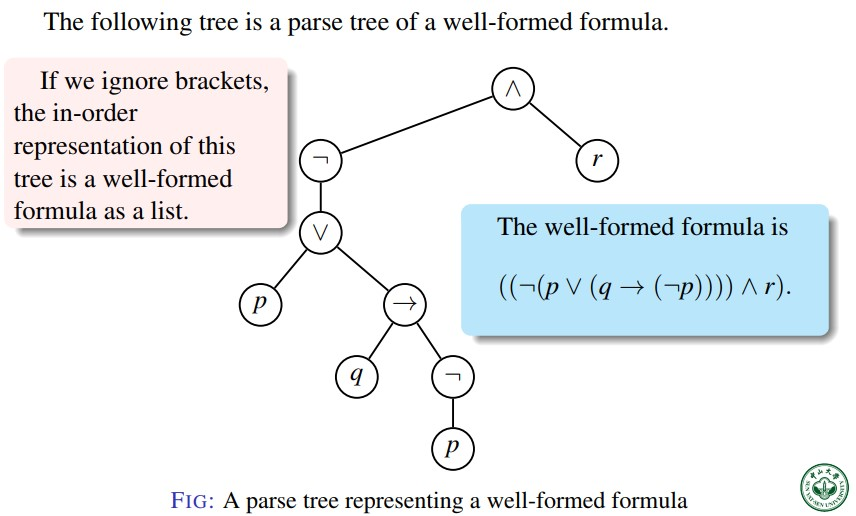
\includegraphics[width=0.8\linewidth]{fig/well-formed_formula.jpg}
\end{figure}
\end{example}

\subsection{语义}
\begin{definition}[模型(model)]
在前提$\phi_1,\phi_2,\ldots,\phi_n$和结论$\psi$上定义另一关系,记作
\[\phi_1,\phi_2,\ldots,\phi_n\models\psi\]
真值包括两个元素$T$和$F$,公式$\phi$的模型(model)或估值(valuation)是指对$\phi$中的每一原子命题都有一个真值指派(assignment)。
对$\phi_1,\phi_2,\ldots,\phi_n$的真值指派决定了$\psi$的真值,称为$\psi$的解释(interpretation),可表示为真值表中的一行。

如果对于所有$\phi_1,\phi_2,\ldots,\phi_n$的估值都为$T$,$\psi$也估值为$T$,那么称
\[\phi_1,\phi_2,\ldots,\phi_n\models\psi\]
成立(hold),且称$\models$为语义后承(semantic entailment)关系。
\end{definition}
\begin{theorem}[可靠性(soundness)]
令$\phi_1,\phi_2,\ldots,\phi_n$和$\psi$都是命题逻辑公式,若$\phi_1,\phi_2,\ldots,\phi_n\vdash\psi$是有效的\footnote{可以由$\phi_1,\ldots,\phi_n$推出$\psi$},那么$\phi_1,\phi_2,\ldots,\phi_n\models\psi$成立。
\end{theorem}
\begin{theorem}[完备性(completeness)]
若$\phi_1,\ldots,\phi_n\models\psi$成立,则存在自然推断证明$\phi_1,\ldots,\phi_n\vdash\psi$。
\end{theorem}
\begin{theorem}
对于命题逻辑来说,完备性和可靠性是等价的。
\end{theorem}

\begin{definition}[恒真式(tautology)/矛盾式(contradiction)]
命题逻辑$\phi$被称为恒真式当且仅当它在所有估值下都取值为$T$,也即$\models\phi$。
若所有估值均为$F$,则为矛盾式。
\end{definition}
\begin{definition}[可满足的(satisfiable)]
令$\phi$为命题逻辑公式,$\phi$是可满足的当且仅当$\lnot\phi$不是有效的。
\end{definition}
\begin{theorem}
若$\models\eta$成立,则$\vdash\eta$是有效的。
换句话说,若$\eta$是永真式,则$\eta$是定理。
\end{theorem}

几个常见逻辑符号的区别\footnote{参考以下资料:
\begin{itemize}
	\item \url{https://math.stackexchange.com/questions/2903877/to-vs-vdash-in-logic}
	\item 逻辑学中,前提为假而命题为真的推论如何解释? - 罗心澄的回答 - 知乎 \url{https://www.zhihu.com/question/21020308/answer/16917222}
	\item 数理逻辑$\implies$,$|$ - 这两个符号有什么区别? - 罗心澄的回答 - 知乎 \url{https://www.zhihu.com/question/21191299/answer/17469774}
	\item 逻辑学蕴涵命题中的$\to$和数学中的$\implies$有什么区别和共同点? - 罗心澄的回答 - 知乎 \url{https://www.zhihu.com/question/276859264/answer/459951353}
\end{itemize}}:
\begin{itemize}
\item \textbf{语义后承}(semantic consequence),符号是$\models$\verb'\models'。
语义后承在一般情况下是连接一个命题集合和一个命题。
如果在任何一种语义赋值$\mM$下,只要命题集合$\Gamma$中的每一个命题都为真(\textbf{真值表}方式),那么$\phi$就一定为真,那么我们就说$\phi$是$\Gamma$的语义后承,记作$\Gamma\models\phi$。
\item \textbf{句法后承}(syntactic consequence),符号是$\vdash$\verb'\vdash'。
句法后承的用法和语义后承类似,也是连接一个命题集合和一个命题,如$\Gamma\vdash\phi$,表示的是$\phi$可以通过\textbf{句法证明}的方式从命题集$\Gamma$中得出。
以Hilbert style的证明为例,这即是说,存在一个命题序列,使得每个前提要么是公理,要么是$\Gamma$中的命题,而这个命题序列的最后一项是$\phi$。
\item \textbf{实质蕴含}(material implication / material conditional),符号是$\to$\verb'\to',当然在强调和不同蕴涵词对比的时候,我们可能会用箭头表示特殊的蕴涵,而用马蹄符号$\supset$表示实质蕴涵,这个取决于作者)。
实质蕴含是一个命题逻辑中的二元算子,连接的是两个命题。
在句法系统中,由Hilbert的前两条公理完全刻画,由第三条公理刻画它和否定的关系。
在语义系统中,我们说$\mM\models\phi\to\psi$当且仅当$\mM\models\psi$或者$\mM\not\models\phi$。
\end{itemize}
可以理解为$\vdash$左侧是一些公理(axiom),右侧是陈述(statement);而$\to$只是一个连接符,本身并不包含推理的信息。
$p\to q$更像是一个数字(如$2+2$),而不是一个判断,它只表达了纯粹的命题内容。
要断定它,更应该说“$p\to q$为真”才行。

\subsection{范式}
\begin{definition}[语义等价(semantic equivalence)]
$\phi$和$\psi$都是命题逻辑的公式,称其等价当且仅当$\phi\models\psi$和$\psi\models\phi$成立,记作$\phi\equiv\psi$,也等价于$\models(\phi\to\psi)\land(\psi\to\phi)$成立,也即同时取真或同时取假。
\end{definition}
\begin{definition}[合取范式(conjunction normal form, CNF)]
BNF定义如下:
\begin{itemize}
	\item 文字(literal):$L::=p\mid\lnot p$
	\item 句子(clause):$D::=L\mid L\lor D$
	\item 公式(formula):$C::=D\mid(D)\mid D\land C$
\end{itemize}
例子如
\[(p \lor r) \land (\lnot p \lor r) \land (p \lor \lnot r)\]
\end{definition}

\begin{definition}[霍尔公式(Horn formula)]
若命题逻辑公式$\phi$能用下面的语法,表示成$H$的一个示例
\[P::=\bot\mid\top\mid p\qquad
A::=P\mid P\land A\qquad
C::=A\to P\qquad
H::=C\mid C\land H\]
则称$C$的每个实例为霍尔子句(clause)。
\end{definition}

\subsection{SAT求解器}
线性求解器只接受以下几种形式的公式
\[\phi::=p\mid(\lnot\phi)\mid(\phi\land\phi)\]
\begin{example}
$\phi=p\land\lnot(q\lor\lnot p)$,计算$T(\phi)=p\land\lnot\lnot(\lnot q\land\lnot\lnot p)$,则有语法树和DAG如下
\begin{figure}[H]
\centering
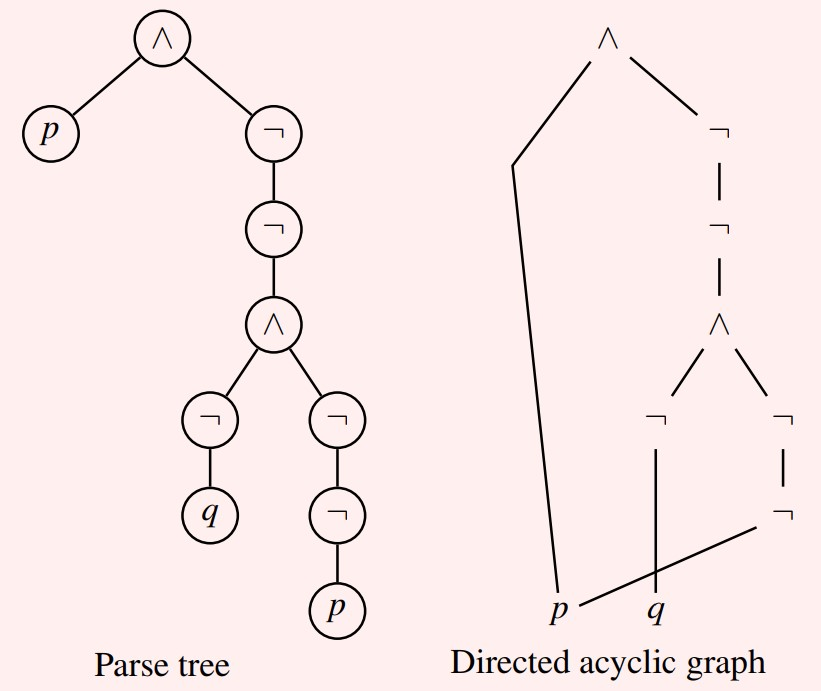
\includegraphics[width=0.5\linewidth]{fig/parse_tree_dag_eg.jpg}
\end{figure}
\end{example}
% !TEX root = main.tex

\section{谓词逻辑}
谓词逻辑(predicate)或被称为一阶逻辑,提供了更强的语言表达能力。

\subsection{形式语言}
\begin{definition}[项(item)]
项的定义如下:
\begin{itemize}
	\item 每一个变量都是项
	\item 若$c\in\mathcal{F}$是一个空函数,则$c$是项(常数)
	\item 若$t_1,t_2,\ldots,t_n$都是项,且$f\in\mathcal{F}$有$n>0$个元(arity),则$f(t_1,t_2,\ldots,t_n)$是一个项
\end{itemize}
用BNF写即
\[t::=x\mid c\mid f(t_1,t_2,\ldots,t_n)\]
\end{definition}
\begin{definition}[公式(formula)]
BNF定义如下
\[\phi::=P(t_1,t_2,\ldots,t_n)\mid
(\lnot\phi)\mid
(\phi\land\psi)\mid
(\phi\lor\psi)\mid
(\phi\to\psi)\mid
(\forall x\phi)\mid
(\exists x\phi)\]
运算符优先级如下
\begin{itemize}
	\item $\lnot,\forall,\exists$
	\item $\lor,\land$
	\item $\to$
\end{itemize}
\end{definition}
\begin{definition}[自由(free)/约束(bound)变量]
语法树叶结点往上不会经过$\forall x$或$\exists x$结点,则为自由变量。
\begin{figure}[H]
\centering
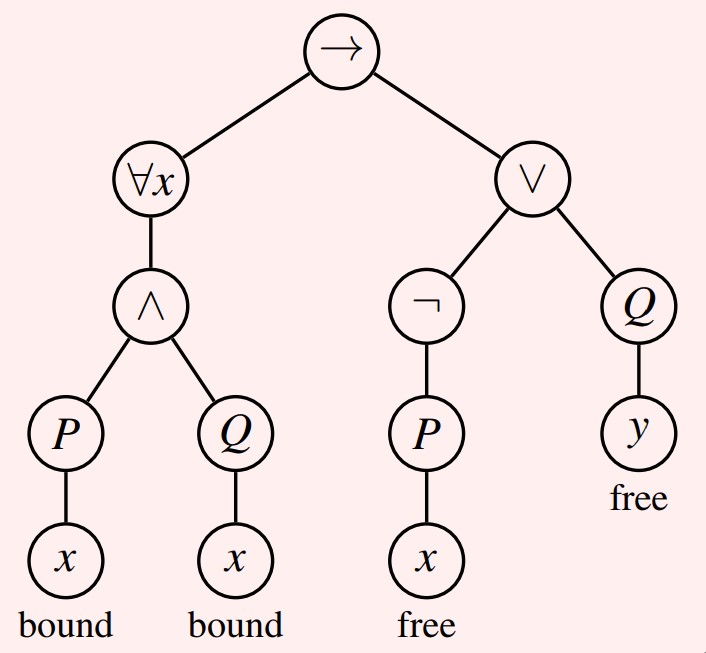
\includegraphics[width=0.4\linewidth]{fig/free_bound_var.jpg}
\end{figure}
\end{definition}
\begin{definition}[替代(substituion)]
给定变量$x$、项$t$和公式$\phi$,定义$\phi[t/x]$为将$\phi$中所有自由$x$用$t$代替
\end{definition}

\subsection{证明论}
\begin{itemize}
	\item equality ($=i$)
	\[\frac{}{t=t}=i\]
	\item substitution ($=e$)
	\[\frac{t_1=t_2\qquad \phi[t_1/x]}{\phi[t_2/x]}=e\]
	\item for-eliminating ($\forall x\quad e$)
	\[\frac{\forall x\phi}{\phi[t/x]}\forall x\quad e\]
	\item for-introduction ($\forall x\quad i$)
	\[\frac{\fbox{\begin{tabular}{c}$x_0$(fresh/dummy var)\\$\vdots$\\$\phi[x_0/x]$\end{tabular}}}{\forall x\phi}\forall x\quad i\]
	\item exists-introduction ($\exists x\quad i$)
	\[\frac{\phi[t/x]}{\exists x\phi}\exists x\quad i\]
	\item exists-elimination ($\exists e$)
	\[\frac{\exists x\phi\quad \fbox{\begin{tabular}{c}$x_0$\quad $\phi[x_0/x]$\\$\vdots$\\$\chi$\end{tabular}}}{\chi}\exists e\]
\end{itemize}
\begin{example}
证明$\forall x(P(x)\to Q(x)),\forall xP(x)\vdash\forall xQ(x)$
\end{example}
\begin{analysis}
推理过程如下
\begin{center}
\begin{tabular}{lll}
1 & $\forall x(P(x)\to Q(x))$ & premise\\
2 & $\forall xP(x)$ & premise\\
3 & $P(x_0)\to Q(x_0)$ & $\forall x\quad e\quad 1$\\
4 & $P(x_0)$ & $\forall x\quad e\quad 2$\\
5 & $Q(x_0)$ & $\to e\quad 3,4$\\
6 & $\forall xQ(x)$ & $\forall x\quad i\quad 3-5$
\end{tabular}
\end{center}
\end{analysis}
\begin{theorem}[等价性(equivalence)]
令$\phi$和$\psi$都为谓词逻辑的公式,有以下等价性
\[\lnot\forall x\phi\dashv\vdash\exists x\lnot\phi,\qquad\lnot\exists x\phi\dashv\vdash\forall x\lnot\phi\]
\end{theorem}

\subsection{语义}
记$\Gamma$为公式$\phi_1,\ldots,\phi_n$,要证明$\Gamma\vdash\psi$是合法的,则只需从$\Gamma$中提供$\psi$的证明。
而如果要证明$\Gamma$推不出$\psi$,从\textbf{证明论}(proof theory)的角度是困难的。

但从语义(semantics)的角度,只需找到一个模型(model)满足所有$\phi_i$都为真,而$\psi$为假,即可得到$\Gamma$推不出$\psi$;相反地,要证明$\Gamma$推出$\psi$则是困难的,因为对于谓词逻辑来说有无穷多种估值/模型,只有全部验证了才能得知$\Gamma\models\psi$($\psi$被$\Gamma$语义蕴含entail)。

因此证明论和模型论两者都是重要的。

\begin{definition}[模型(model)]
令$\mathcal{F}$为函数符号的集合,$\mathcal{P}$为谓词符号的集合\footnote{函数符号是一个算子,作用在项上并生成一个新的项/实体(object),比如$+$和$\times$;而谓词符号也是一个算子,作用在项上并生成一个谓词/宣称(claim),比如$<$和$>$。}。
关于$(\mathcal{F},\mathcal{P})$的模型$\mathcal{M}$包含以下数据:
\begin{itemize}
	\item 非空集合$A$:具体值的全集
	\item 对于每一空函数符号$f\in\mathcal{F},f^{\mathcal{M}}\in A$
	\item 对于每一$f\in\mathcal{F}$且元$n>0$,具体函数$f^{\mathcal{M}}:A^n\to A$
	\item 对于每一$P\in\mathcal{P}$且元$n>0$,子集$P^\mathcal{M}\subset A^n$
\end{itemize}
也就是说$f$和$P$仅仅是\textbf{抽象的符号},而$f^{\mathcal{M}}$和$P^{\mathcal{M}}$为\textbf{具体的函数/元素}。\\
也可以说模型给出了一个解释(interpretation)。
\end{definition}
\begin{example}
令$\mF\eqdef\{i\}$,$\mP\eqdef\{R,F\}$,其中$i$是一个常数,$F$是一元谓词符号,$R$是二元谓词符号。
一个模型可以是
\[\begin{aligned}
A &\eqdef\{a,b,c\}\\
i^{\mM} &\eqdef a\\
R^{\mM} &\eqdef\{(a,a),(a,b),(a,c),(b,c),(c,c)\}\\
F^{\mM} &\eqdef\{b,c\}
\end{aligned}\]
那么有$\exists yR(i,y)$为真,$\lnot F(i)$为真。
\end{example}

上面给出了模型的定义,并且使得我们可以直接从$(\mathcal{F},\mathcal{P})$中计算出真值,但我们仍需讨论如何处理全称量词$\forall x\phi$及特称量词$\exists x\phi$,需要检查$\phi$是否对于所有模型中的$a$都成立。
尽管我们可以用$\phi[a/x]$表示,但是$\phi[a/x]$并不是一个逻辑公式,因为$a$不是一个项(term)而是模型中的一个元素。

因此需要限定公式是关于一个环境的(relative to an environment)。
\begin{definition}[环境(environment)/查找表(look-up table)]
对于全集$A$具体值的环境是一个函数$l:var\to A$,定义$l[x\mapsto a]$为从$x$映射到$a$的查找表。
\end{definition}

\begin{definition}[满足关系(satisfaction)]
给定$\mathcal{M}(\mF,\mP)$及环境$l$,定义满足关系$\mM\models_l\phi$。
若$\mM\models_l$成立(hold),则称$\phi$在关于环境$l$的模型$\mM$中计算为$T$。
\end{definition}

\begin{example}
令$F\eqdef\{alma\},P\eqdef\{loves\}$,其中$alma$是常数,$loves(\cdot,\cdot)$是谓词符号。
模型$\mM$包含集合
\[A\eqdef\{a,b,c\},alma^\mM\eqdef a,loves^\mM\eqdef\{(a,a),(b,a),(c,a)\}\]
检查模型$\mM$是否满足
\[\text{None of Alma's lovers' lovers love her.}\]
\[\phi:\forall x\forall y(loves(x,alma)\land loves(y,x)\to\lnot loves(y,alma))\]
令$x\mapsto a$及$y\mapsto b$,又$alma^{\mM}\eqdef a$,得到
\[loves(a,a)\land loves(b,a)\to\lnot loves(b,alma)\]
不成立,故$\mM\not\models\phi$
\end{example}

在命题逻辑中,$\phi_1,\ldots,\phi_n\models\psi$\footnote{$\models$代表语义蕴含(semantic entailment)}当且仅当$\phi_1,\ldots,\phi_n$都估值为$T$,同时$\psi$也估值为$T$。

\begin{definition}
令$\Gamma$为谓词逻辑的公式集合,$\psi$为谓词逻辑的公式
\begin{enumerate}
	\item 语义蕴含$\Gamma\models\psi$成立当且仅当对于\textbf{所有}的模型$\mM$和查找表$l$,只要$\forall \phi\in\Gamma:\mM\models_l\phi$成立,$\mM\models_l\psi$也成立
	\item $\psi$是可满足的(satisfiable)当且仅当\textbf{存在}模型$\mM$和环境$l$使得$\mM\models_l\psi$成立
	\item $\psi$是合法的(valid)当且仅当$\mM\models_l\psi$对于\textbf{所有}模型$\mM$和环境$l$都成立
\end{enumerate}
\end{definition}
\begin{example}
考虑以下语义蕴含关系
\[\forall x(P(x)\to Q(x))\models\forall xP(x)\to\forall xQ(x)\]
令$\mM$为满足$\forall x(P(x)\to Q(x))$的模型,需要证明$\mM$也满足$\forall xP(x)\to\forall xQ(x)$
\begin{itemize}
	\item 若不是每个$\mM$中的元素都满足$P$,则前件为假,显然成立
	\item 若每个$\mM$中的元素都满足$P$,则每一元素都满足$Q$,因为$\mM$满足$\forall x(P(x)\to Q(x))$
\end{itemize}
进而$\mM\models\forall xP(x)\to\forall xQ(x)$
\end{example}
\begin{example}
考虑以下语义蕴含关系
\[\forall xP(x)\to\forall xQ(x)\models\forall x(P(x)\to Q(x))\]
令$A\eqdef\{a,b\},P^\mM\eqdef\{a\},Q^\mM\eqdef\{b\}$,则$\mM\models\forall xP(x)\to\forall xQ(x)$,但$\mM\not\models\forall x(P(x)\to Q(x))$
\end{example}

% \subsection{不可判定性}
% !TEX root = main.tex

\section{模型验证}
\subsection{线性时序逻辑}
\begin{definition}[线性时序逻辑(linear-time temporal logic, LTL)]
BNF定义如下
\[\phi::=\top\mid\bot\mid p\mid
(\lnot\phi)\mid
(\phi\land\phi)\mid
(\phi\lor\phi)\mid
(\phi\to\phi)\mid
(X\phi)\mid
(F\phi)\mid
(G\phi)\mid
(\phi U\phi)\mid
(\phi W\phi)\mid
(\phi R\phi)\]
其中$X,F,G,U,R,W$都称为时序连接词(temporal connectives)
\begin{itemize}
	\item $X$:neXt state
	\item $F$:some Future state(存在)
	\item $G$:all future states (Globally)(任意)
	\item $U$:Until(二元)
	\item $R$:Release(二元)
	\item $W$:Weak-until(二元)
\end{itemize}
运算符优先级
\begin{itemize}
	\item 一元连接词:$\lnot,X,F,G$
	\item $U,R,W$
	\item $\land,\lor$
	\item $\to$
\end{itemize}
\end{definition}
\begin{definition}[转移系统(transition system)]
一个转移系统$\mM=(S,\to,L)$是状态集合$S$(静态结构),转移关系$\to$(动态结构),使得$\forall s\in S,\exists s'\in S:\;s\to s'$,且有标注函数$L:S\to\mathcal{P}(Atoms)$,其中$\mP(Atoms)$为原子描述的幂集(实际上$L$就是给所有命题原子做真值指派)。
转移系统也可以被称作模型(model)。
\end{definition}
\begin{figure}[H]
\centering
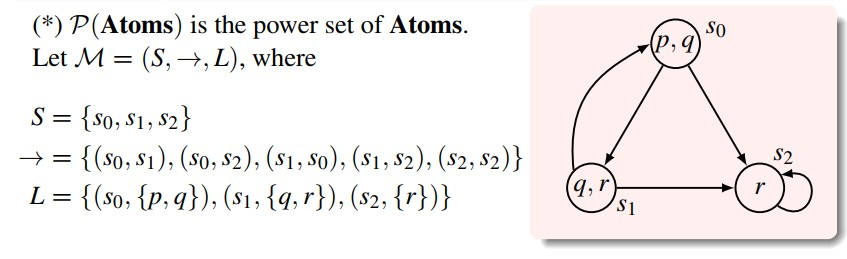
\includegraphics[width=0.8\linewidth]{fig/transition_system.jpg}
\end{figure}
\begin{definition}[路径(path)]
路径是一个无穷序列$s_1,s_2,\ldots\in S$使得$s_i\to s_{i+1},\forall i\geq 1$。
令$\pi^i=s_i\to s_{i+1}\to\cdots$为从状态$s_i$开始的路径。
路径$\pi=s_1\to s_2\to\cdots$满足LTL公式定义在满足关系$\models$上:
\begin{enumerate}
	\item $\pi\models\top$
	\item $\pi\not\models\bot$
	\item $\pi\models p$ iff $p\in L(s_1)$
	\item $\pi\models\lnot\phi$ iff $\pi\not\models\phi$
	\item $\pi\models\phi\land\psi$ iff $\pi\models\phi$ and $\pi\models\psi$
	\item $\pi\models\phi\lor\psi$ iff $\pi\models\phi$ or $\pi\models\psi$
	\item $\pi\models\phi\to\psi$ iff $\pi\models\psi$ when $\pi\models\phi$
	\item $\pi\models X\phi$ iff $\pi^2\models\phi$
	\item $\pi\models G\phi$ iff $\forall i\geq 1:\;\pi^i\models\phi$
	\item $\pi\models F\phi$ iff $\exists i\geq 1:\;\pi^i\models\phi$
	\item $\pi\models \phi U\psi$ iff $\exists i\geq 1:\;\pi^i\models\psi$ and $\forall j=1,\ldots,i-1:\;\pi^j\models\phi$
	\item $\pi\models \phi W\psi$ iff \textbf{either} $\exists i\geq 1:\;\pi^i\models\psi$ and $\forall j=1,\ldots,i-1:\;\pi^j\models\phi$ \textbf{or} $\forall k\geq 1:\;\pi^k\models\phi$
	\item $\pi\models \phi R\psi$ iff \textbf{either} $\exists i\geq 1:\;\pi^i\models\phi$ and $\forall j=1,\ldots,i:\;\pi^j\models\psi$ \textbf{or} $\forall k\geq 1:\;\pi^k\models\psi$
\end{enumerate}
记$\mM,s\models\phi$表示对于所有$\mM$开始于$s$的执行路径$\pi$,都有$\pi\models\phi$,或可简写为$s\models\phi$
\end{definition}
注意有以下恒等式
\[\begin{aligned}
\lnot G\phi&\equiv F\lnot\phi\\
\lnot F\phi&\equiv G\lnot\phi\\
\lnot X\phi&\equiv X\lnot\phi\\
\phi W\psi&\equiv \phi U\psi\lor G\phi\\
\phi R\psi&\equiv \lnot(\lnot\phi U\lnot\psi)\\
F(\phi\lor\psi)&\equiv F\phi\lor F\psi\\
G(\phi\land\psi)&\equiv G\phi\land G\psi\\
F\phi&\equiv\top U\phi\\
G\phi&\equiv\bot R\phi\\
\phi U\psi&\equiv\phi W\psi\land F\psi\\
\phi W\psi&\equiv\phi U\psi\lor G\phi\\
\phi W\psi&\equiv\psi R(\phi\lor\psi)\\
\phi R\psi&\equiv\psi W(\phi\land\psi)
\end{aligned}\]
\begin{example}
对于上图的例子,有以下式子成立
\begin{itemize}
	\item $s_0\models p\land q$ (3,5)
	\item $s_0\models X r$,因$r\in L(s_1),L(s_2)$
	\item $s_0\models G\lnot (p\land r)$,因所有从$s_0$开始的路径都满足$G\lnot(p\land r)$,也即满足$\lnot(p\land r)$
\end{itemize}
\end{example}

\subsection{模型检查}
下面是一个互斥锁的例子,$n$为非临界区状态,$t$为尝试进入临界区,$c$为临界区状态。
考虑2个进程,每个进程的转移都是$n\to t\to c\to n\to\cdots$。
\begin{figure}[H]
\centering
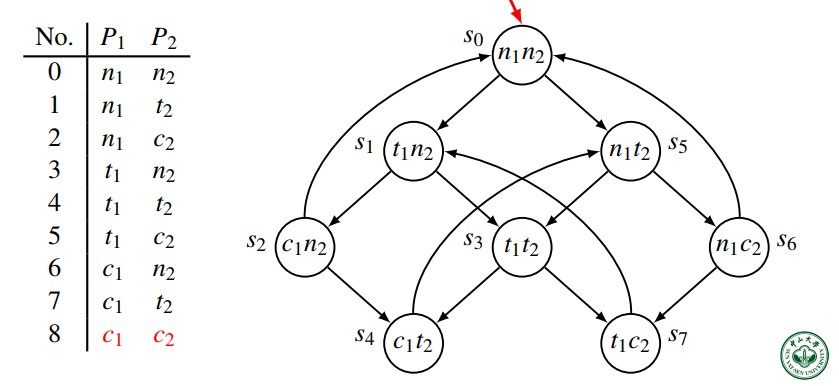
\includegraphics[width=0.8\linewidth]{fig/mutual_exclusion.jpg}
\end{figure}
有以下性质:
\begin{itemize}
	\item 安全性(safety):$G\lnot(c_1\land c_2)$在每个状态都被满足
	\item 活性(liveness):$G(t_1\to Fc_1)$,对于路径$s_0\to s_1\to s_3\to s_7\to s_1\to s_3\to\cdots$就不满足
	\item 非阻塞(non-blocking):对于任意状态满足$n_1$,有后继状态满足$t_1$,无法用LTL表达
	\item 非严格序列(strict sequencing)
\end{itemize}

\subsection{计算树逻辑}
\begin{definition}[计算树逻辑(computation tree logic, CTL)]
除了LTL有的$U,F,G,X$,CTL还有$A$和$E$表示\textbf{所有}路径(All path)和\textbf{存在}一条路径(Exist a path)。
BNF定义如下
\[\begin{aligned}
\phi::=&\top\mid\bot\mid p\mid
(\lnot\phi)\mid
(\phi\land\phi)\mid
(\phi\lor\phi)\mid
(\phi\to\phi)\mid
(AX\phi)\mid
(EX\phi)\mid\\
&(AF\phi)\mid
(EF\phi)\mid
(AG\phi)\mid
(EG\phi)\mid
A[\phi U\phi]\mid
E[\phi U\phi]
\end{aligned}\]
运算符优先级
\begin{itemize}
	\item $\lnot,AG,EG,AF,EF,AX,EX$
	\item $\land,\lor$
	\item $\to,AU,EU$
\end{itemize}
\end{definition}
\begin{definition}[CTL*]
$\phi$为状态公式(在状态上求值),$\alpha$为路经公式(在路径上求值)
\[\begin{aligned}
\phi&::=
\top\mid
p\mid
(\lnot\phi)\mid
(\phi\land\phi)\mid
A[\alpha]\mid
E[\alpha]\\
\alpha&::=\phi\mid
(\lnot\alpha)\mid
(\alpha\land\alpha)\mid
(\alpha U\alpha)\mid
(G\alpha)\mid
(F\alpha)\mid
(X\alpha)
\end{aligned}\]
\end{definition}
\begin{figure}[H]
\centering
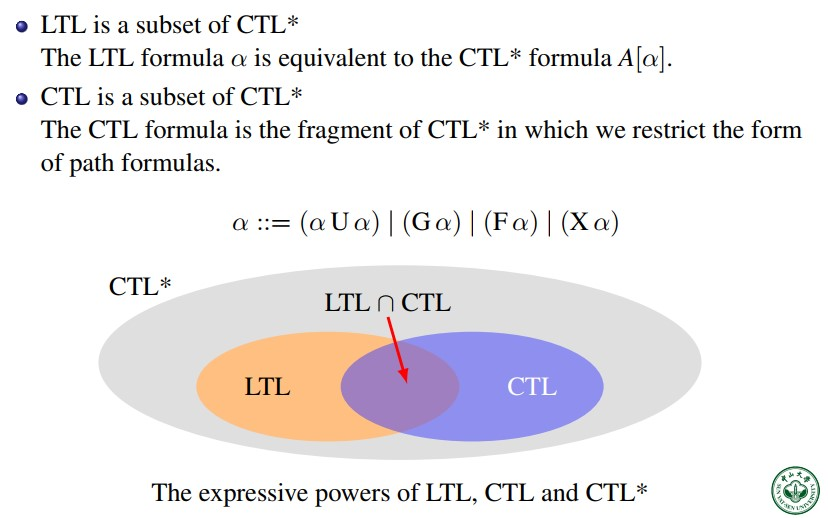
\includegraphics[width=0.8\linewidth]{fig/ltl_ctl.jpg}
\end{figure}
% !TEX root = main.tex

\section{程序验证}
\begin{definition}[霍尔三元组(Hoare triple)]
\[\hoare{\phi}P\hoare{\psi}\]
代表若程序$P$在满足$\phi$的状态下运行,则执行完$P$的状态会满足$\psi$。
$\phi$称为先验条件(precondition),$\psi$称为后验条件(postcondition)。
存储变量$x$记为$l(x)$。
\end{definition}
\begin{example}
若输入$x$是正数,则求出一个数字它的平方小于$x$。\\
记程序为$P$,则Hoare三元组为
\[\hoare{x>0}P\hoare{y\cdot y<x}\]
一个可行的程序$P$可以是
\begin{lstlisting}
y = 0;
while (y * y < x) { y = y + 1; }
y = y - 1;
\end{lstlisting}
\end{example}
\begin{definition}[部分正确性(partial correctness)]
若对于\textbf{所有}满足先验条件$\phi$的状态,\textbf{只要$P$需要能停止(terminate)},经过$P$的执行,都满足后验条件$\psi$,则$\hoare{\phi}P\hoare{\psi}$满足部分正确性。
若$\models_{par}\hoare{\phi}P\hoare{\psi}$成立,则称$\models_{par}$为部分正确性关系。
全部正确性(total correctness)则是保证了$P$一定会停止。
\end{definition}
\begin{example}
考虑下面求阶乘的程序Fac1:
\begin{lstlisting}
y = 1;
z = 0;
while (z != x) {
  z = z + 1;
  y = y * z;
}
\end{lstlisting}
\begin{itemize}
\item $\models_{tot}\hoare{x \geq 0 } Fac1\hoare{y = x! }$成立,只要$x \geq 0$,Fac1一定会停止,并且有结果$y = x!$
\item $\models_{tot}\hoare{\top } Fac1\hoare{y = x! }$不保证成立,因为Fac1对于$x$的负数值不会停止
\item $\models_{par}\hoare{x \geq 0 } Fac1\hoare{y = x! }$和$\models_{par}\hoare{\top} Fac1\hoare{y = x!}$成立
\end{itemize}
\end{example}
\begin{definition}[逻辑变量(logical variable)]
逻辑变量在$\phi$或$\psi$是自由的,且不出现在$P$中
\end{definition}
\begin{example}
$\hoare{x=x_0\land x\geq 0}Sum\hoare{z=x_0(x_0+1)/2}$
\begin{lstlisting}
z = 0;
while (x != 0) {
  z = z + x;
  x = x - 1;
}
\end{lstlisting}
\end{example}

\subsection{证明论}
\begin{itemize}
	\item Composition
	\[\frac{\htriple{\phi}{C_1}{\eta}\qquad\htriple{\eta}{C_2}{\psi}}{\htriple{\phi}{C_1;C_2}{\psi}}\]
	\item Assignment
	\[\frac{}{\htriple{\psi[E/x]}{x=E}{\psi}}\]
	注意这条公式相当tricky,是在先验条件中将$x$换为$E$(即恢复$x=E$的赋值),在具体证明中往往是反过来用
	\item If-statement
	\[\frac{\htriple{\phi\land B}{C_1}{\psi}\qquad\htriple{\phi\land\lnot B}{C_2}{\psi}}{\htriple{\phi}{\text{if }B\{C_1\}\text{ else }\{C_2\}}{\psi}}\]
	\item Partial-while
	\[\frac{\htriple{\psi\land B}{C}{\psi}}{\htriple{\psi}{\text{while }B\{C\}}{\psi\land\lnot B}}\]
	\item Implied
	\[\frac{\vdash_{AR}\phi'\to\phi\qquad\htriple{\phi}{C}{\psi}\qquad\vdash_{AR}\psi\to\psi'}{\htriple{\phi'}{C}{\psi'}}\]
	基本谓词逻辑演算及算术表达都满足
\end{itemize}
\begin{example}[表格证明(proof tableaux)]
$\vdash_{par}\htriple{y<3}{y=y+1}{y<4}$
\[\begin{array}{ll}
\hoare{y<3} &\\
\hoare{y+1 < 4} & \text{Implied}\\
y = y+1 &\\
\hoare{y<4} &\text{Assignment}
\end{array}\]
\end{example}

\[\htriple{\phi}{\text{if }(B)\{C_1\}\text{ else }\{C_2\}}{\psi}\]
\begin{itemize}
	\item 将$\psi$反推$C_1$,结果记为$\phi_1$
	\item 将$\psi$反推$C_2$,结果记为$\phi_2$
	\item 令$\phi=(B\to\phi_1)\land(\lnot B\to\phi_2)$
\end{itemize}
\begin{example}
考虑程序$Succ$
\begin{lstlisting}
a = x + 1;
if (a-1 == 0) { y = 1; } else { y = a; }
\end{lstlisting}
证明$\vdash_{par}\htriple{\top}{Succ}{y=x+1}$合法
\end{example}
\begin{analysis}
可以自底向上分析
\begin{lstlisting}[language=c++]
  `\textcolor{red}{$\hoare{\top}$}'
  `\textcolor{red}{$\hoare{(x+1-1=0\to1=x+1)\land(\lnot(x+1-1=0)\to x+1=x+1)}$ Implied}'
a = x + 1;
  `\textcolor{red}{$\hoare{(a-1=0\to 1=x+1)\land(\lnot(a-1=0)\to a=x+1)}$ Assignment}'
if (a - 1 == 0) {
    `\textcolor{red}{$\hoare{1=x+1}$ If-statements}'
  y = 1;
    `\textcolor{red}{$\hoare{y=x+1}$ Assignment}'
} else {
    `\textcolor{red}{$\hoare{a=x+1}$ If-statements}'
  y = a;
    `\textcolor{red}{$\hoare{y=x+1}$ Assignment}'
}
    `\textcolor{red}{$\hoare{y=x+1}$ If-statements}'
\end{lstlisting}
\end{analysis}

\[\htriple{\phi}{\text{while }B\{C\}}{\psi}\]
需要找到合适的不变量(invariant)$\eta$使得
\begin{itemize}
	\item $\models_{AR}\phi\to\eta$
	\item $\models_{AR}\eta\land\lnot B\to\psi$
	\item $\models_{par}\hoare{\eta}$ while $(B)\{C\}\hoare{\eta\land\lnot B}$
\end{itemize}
\begin{example}
考虑程序$Fac1$
\begin{lstlisting}[language=c++]
y = 1;
z = 0;
while (z != x) { // L1
  z = z + 1;
  y = y * z;
} // L2
\end{lstlisting}
证明
\[\models_{AR}(y=1\land z=0)\to(y=z!)\qquad
\models_{AR}(y=z!\land x=z)\to(y=x!)\]
\begin{lstlisting}[language=c++]
  `\textcolor{red}{$\hoare{\top}$}'
  `\textcolor{red}{$\hoare{1=0!}$ Implied}'
y = 1;
  `\textcolor{red}{$\hoare{y=0!}$ Assignment}'
z = 0;
  `\textcolor{red}{$\hoare{y=z!}$ Assignment}'
while (z != x) {
    `\textcolor{red}{$\hoare{y=z!\land z\ne x}$ Invariant Hyp. $\land$ guard}'
    `\textcolor{red}{$\hoare{y\cdot(z+1)=(z+1)!}$ Implied}'
  z = z + 1;
    `\textcolor{red}{$\hoare{y\cdot z=z!}$ Assignment}'
  y = y * z;
    `\textcolor{red}{$\hoare{y=z!}$ Assignment}'
}
  `\textcolor{red}{$\hoare{y=z!\land\lnot(z\ne x)}$ Partial-while}'
  `\textcolor{red}{$\hoare{y=x!}$ Implied}'
\end{lstlisting}
\end{example}
% !TEX root = main.tex

\section{模态逻辑}
\begin{definition}[模态逻辑(modal logic)]
BNF定义如下
\[\phi::=\top\mid
\bot\mid
p\mid
(\lnot\phi)\mid
(\phi\land\phi)\mid
(\phi\lor\phi)\mid
(\phi\to\phi)\mid
(\phi\leftrightarrow\phi)\mid
(\square\phi)\mid
(\Diamond\phi)\]
其中$\square$为一定(necessarily),$\Diamond$为可能(possibly)。
优先级顺序
\begin{itemize}
	\item $\lnot,\square,\Diamond$
	\item $\lor,\land$
	\item $\to,\leftrightarrow$
\end{itemize}
\end{definition}
\begin{definition}[模型(model)]
模态逻辑的模型$\mM$由以下三个成分定义:
\begin{itemize}
	\item 世界(world)元素$W$
	\item 定义在$W$上的可访问(accessibility)关系$R\subset W\times W$
	\item 标记函数(labeling)$L:W\to\mathcal{P}(Atoms)$
\end{itemize}
这些模型称为Kripke模型
\end{definition}
\begin{figure}[H]
\centering
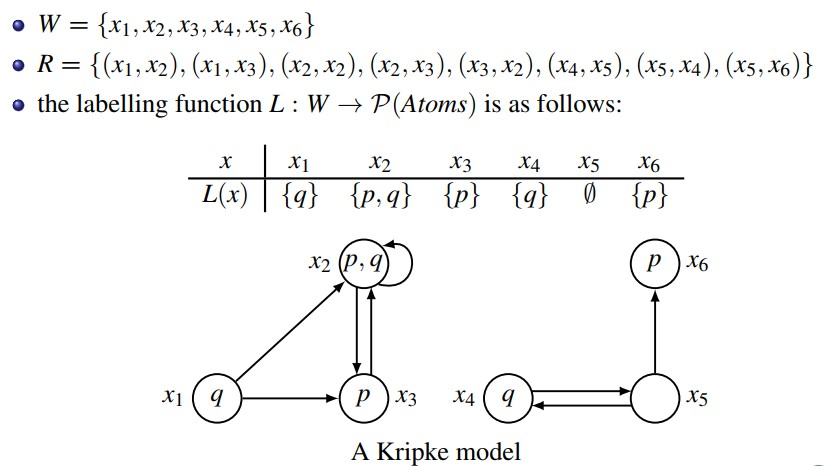
\includegraphics[width=0.8\linewidth]{fig/kripke_model.jpg}
\end{figure}

\begin{definition}
令$\mM=(W,R,L)$为基本的模态逻辑,$x\in W$和$\phi$是公式,满足性(satisfaction)关系$x\Vdash\phi$为在$\phi$上的结构推断(structural induction):
\[\begin{array}{rll}
x & \Vdash\top\\
x & \not\Vdash\bot\\
x & \Vdash p & \text{iff } p\in L(x)\\
x & \Vdash\lnot\phi & \text{iff } x\not\Vdash\phi\\
x & \Vdash\phi\land\psi & \text{iff } x\Vdash\phi \text{ and } x\Vdash\psi\\
x & \Vdash\phi\lor\psi & \text{iff } x\Vdash\phi \text{ or } x\Vdash\psi\\
x & \Vdash\phi\to\psi & \text{iff } x\Vdash\psi \text{ whenever } x\Vdash\phi\\
x & \Vdash\phi\leftrightarrow\psi & \text{iff } (x\Vdash\phi \text{ iff } x\Vdash\psi)\\
x & \Vdash\square\psi & \text{iff }\forall y\in W, R(x,y):\; y\Vdash\psi\\
x & \Vdash\Diamond\psi & \text{iff }\exists y\in W, R(x,y):\; y\Vdash\psi
\end{array}\]
\end{definition}
\begin{example}
比如上图的例子有
\begin{itemize}
	\item $x_1\Vdash q$,因$q\in L(x_1)$
	\item $x_1\Vdash\Diamond q$,因$R(x_1)=\{x_2,x_3\},x_2\in R(x_1),q\in L(x_2)$
	\item $x_1\not\Vdash\square q$,因$R(x_1)=\{x_2,x_3\},x_3\in R(x_1),q\notin L(x_3)$
\end{itemize}
\end{example}

De Morgan定律
\[\lnot\square\phi\equiv\Diamond\lnot\phi\qquad
\lnot\Diamond\phi\equiv\square\lnot\phi\]
分配律
\[\square(\phi\land\psi)\equiv\square\phi\land\square\psi\qquad
\Diamond(\phi\lor\psi)\equiv\Diamond\phi\lor\Diamond\psi\]
K模式(scheme)
\[\square(\phi\to\psi)\land\square\phi\to\square\psi\]
\begin{example}
证明$\lnot\square\phi\equiv\Diamond\lnot\phi$
\end{example}
\begin{analysis}
假设$x$是模型$\mM=(W,R,L)$的一个世界,希望找到$x\Vdash\lnot\square\phi\leftrightarrow\Diamond\lnot\phi$
\[\begin{aligned}
& x\Vdash\lnot\square\phi\\
\leftrightarrow & \text{it is not the case that } x\Vdash\square\phi\\
\leftrightarrow & \text{it is not the case that } \forall y\in R(x), y\Vdash\phi\\
\leftrightarrow & \exists y\in R(x)\text{ and not }y\Vdash\phi\\
\leftrightarrow & \exists y\in R(x)\text{ and }y\Vdash\lnot\phi\\
\leftrightarrow & x\Vdash\Diamond\lnot\phi
\end{aligned}\]
\end{analysis}
% !TEX root = main.tex

\section{二元决策图}
$\cdot$为与,$+$为或,$\oplus$为异或。

布尔函数用真值表表示,如$f(x,y)\eqdef\overline{x+y}$。
\begin{center}
\begin{tabular}{cc|c}
$x$ & $y$ & $f(x,y)$\\\hline
$1$ & $1$ & $0$ \\
$1$ & $0$ & $1$ \\
$0$ & $1$ & $0$ \\
$0$ & $0$ & $1$
\end{tabular}
\end{center}

二元决策图(Binary Decision Diagram, BDD)
\begin{itemize}
	\item 非终端结点标号为布尔变量
	\item 终端结点(叶子)标号为0或1
	\item 每一个非终端结点有两条边,一条虚边(dashed)指向0,一条实边(solid)指向1
\end{itemize}

简化法则:
\begin{itemize}
	\item 去除重复终端(terminal)
	\item 去除冗余测试:若结点$n$出边都指向同个结点$m$,则消除$n$
	\item 去除重复非终端符号:第一条是本条的特例
\end{itemize}
\begin{figure}[H]
\centering
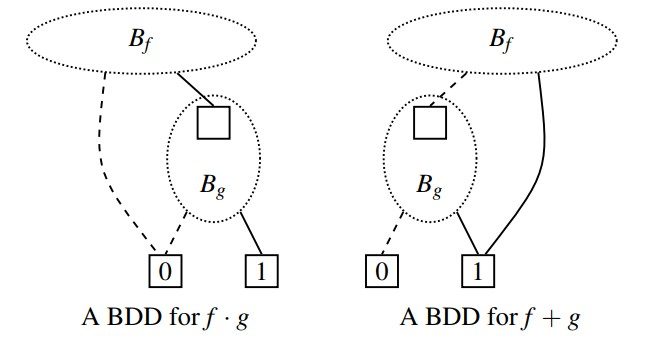
\includegraphics[width=0.8\linewidth]{fig/shortcut_bdd.jpg}
\end{figure}

\begin{definition}[有序BDD]
令$[x_1,\ldots,x_n]$为有序$n$个变量,$B$为含有这些变量的BDD
\begin{itemize}
	\item 令$V(B)$为OBDD的变量集,即$V(B)=\{x_1,x_2,\ldots,x_n\}$
	\item $O_B(x_i)$是$\forall x_i\in V(B)$的序
	\item $\forall x_i,x_j\in V(B),O_B(x_i)<O_B(x_j)$为在$B$中任一路径每一个$x_i$跟随$x_j$
\end{itemize}
\end{definition}

\subsection{约简规则}
\begin{definition}
给定BDD中非终端结点$n$
\begin{itemize}
	\item $lo(n)$是从$n$用虚线指向的点
	\item $hi(n)$是从$n$用实线指向的点
\end{itemize}
$id(\cdot)$为结点编号
\end{definition}

\begin{figure}[H]
\centering
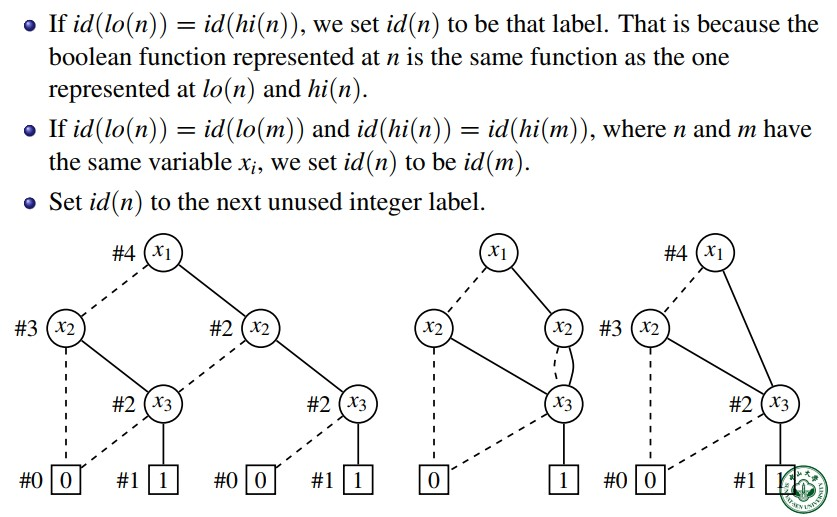
\includegraphics[width=0.8\linewidth]{fig/reduce_alg.jpg}
\end{figure}

\subsection{应用规则}
\begin{definition}[香农展开(Shannon expansion)]
对于所有布尔公式$f$及布尔变量$x$(包括那些不出现在$f$中的),有
\[f\equiv\bar{x}\cdot f[0/x]+x\cdot f[1/x]\]
\end{definition}
应用(apply)函数基于$f \op g$的展开
\[\begin{aligned}
f \op g &\equiv(\bar{x}\cdot f[0/x]+x\cdot f[1/x])\op(\bar{x}\cdot g[0/x]+x\cdot g[1/x])\\
&\equiv(\bar{x}\cdot f[0/x]\op\bar{x}\cdot g[0/x])+(x\cdot f[1/x]\op x\cdot g[1/x])\\
&\equiv\bar{x}\cdot(f[0/x]\op g[0/x])+x\cdot(f[1/x]\op g[1/x])
\end{aligned}\]

\begin{itemize}
\item 特称规则:
\[\exists x.f\eqdef f[0/x]+f[1/x]\]
\item 全称规则:
\[\exists x.f\eqdef f[0/x]\cdot f[1/x]\]
\end{itemize}

\begin{center}
\begin{tabular}{c|l|c|l}
$f$ & OBDD $B_f$ & $f$ & OBDD $B_f$\\\hline
$0$ & $B_0$ & $1$ & $B_1$\\
$x$ & $B_x$ & $\bar{f}$ & 交换$B_f$中的0和1结点\\\hline
$f+g$ & $apply(+,B_f,B_g)$ & $f\cdot g$ & $apply(\cdot,B_f,B_g)$\\
$f\oplus g$ & $apply(\oplus,B_f,B_g)$ & &\\
$f[0/x]$ & $restrict(0,x,B_f)$ & $f[1/x]$ & $restrict(1,x,B_f)$\\\hline
$\exists x.f$ & $apply(+,B_{f[0/x]},B_{f[1/x]})$ & $\forall x.f$ & $apply(\cdot,B_{f[0/x]},B_{f[1/x]})$
\end{tabular}
\end{center}

\end{document}